%************************************************
\chapter{Grundlagen}\label{ch:grundlagen}
%************************************************

\section{Softwarewartung nach ISO/IEC 14764}
Die \ac{ISO} ist ein im Jahr 1947 gegründeter Zusammenschluss internationaler Normungskommissionen, mit dem Ziel internationale Standards zu entwickeln und zu etablieren.\cite{international_organization_for_standardization:_about_nodate}
Die Entwicklung von Standards wird von der 1906 gegründeten Schwesterorganisation \ac{IEC} übernommen, oftmals in Zusammenarbeit mit der \ac{ISO}.\cite{international_electrotechnical_commission_iec_nodate}
Aus dieser Zusammenarbeit entstandene Standards tragen die Kürzel beider Organisationen im Namen. Ein solcher Standard ist \textbf{ISO/IEC 14764} mit dem Titel
\textbf{Software Engineering — Software Life Cycle Processes — Maintenance}, der erstmals im Jahr 1999 veröffentlicht wurde.
\textbf{ISO/IEC 14764} normiert den Prozess der Wartung von Software bis zu deren Einstellung.
Darin wird unter Anderem beschrieben, welche Schritte bei der Migration von Software zu befolgen sind, sobald diese an eine neue Umgebung angepasst werden muss.
Folgende Aktionen sind durch den Ausführenden nach \textbf{ISO/IEC 14764} umzusetzen:
\begin{itemize}
    \item Analyse der Anforderungen und Definition der Migration
    \item Entwicklung von Werkzeugen zur Migration
    \item Entwicklung der an die neue Umgebung angepassten Software
    \item Durchführung der Migration
    \item Verifikation der Migration
    \item Support der alten Umgebung
\end{itemize}

\section{Die Programmiersprache PHP}
\ac{PHP} ist eine Skriptsprache, welche seit 1994 entwickelt wird und seit 1995 Open-Source bereitgestellt wird.
Obwohl \ac{PHP} viele Einsatzzwecke abdeckt, wird es hauptsächlich dazu genutzt, dynamische Websites zu programmieren. 
Rasmus Lerdorf, der Erfinder von \ac{PHP}, entwickelte zunächst eine Reihe von \acp{CGI} in \textit{C}, um die Anzahl der 
Besucher seiner Webseite zu erfassen. Diese \acp{CGI} wurden immer umfangreicher, wodurch sich im Laufe der Zeit eine 
eigenständige Programmiersprache entwickelte, die durch den \textbf{Zend-Engine} genannten Compiler interpretiert wird.
\ac{PHP} steht auf Platz 6 der beliebstesten Programmiersprachen weltweit\cite{carbonnelle_pypl_2019} und ist die Grundlage
für bekannte Projekte wie das Content Management System \textit{Wordpress}\footnote{Wordpress, \url{https://wordpress.org}}
oder die e-Commerce Plattform \textit{Magento}\footnote{Magento, \url{https://magento.com}}.

\section{Versionierung von Software}
Für die Benennung von Releases einer Software gibt es keinen einheitlichen Standard. Jedem Entwickler steht es frei, seine
Software nach einem bestimmten Muster zu benennen. So benennt \textit{Canonical} das Betriebssystem Ubuntu stets nach der 
Jahres- und Monatszahl der Veröffentlichung (bspw. erschien Ubuntu 19.10 im Oktober 2019). \ac{PHP} hingegen implementiert
lose die Spezifikation \textit{Semantic Versioning 2.0.0}. Diese legt ein Muster für Versionsnummern fest, das 
folgendermaßen aufgebaut ist: \\
Die Versionsnummer folgt immer dem Muster \\ \centerline{\textbf{Major}.\textbf{Minor}.\textbf{Patch}{[-\textbf{Pre-Release}]}}
Mit jedem Release wird eine der Nummern inkrementiert, wobei die nachfolgenden Nummern auf ,,0`` zurückgesetzt werden 
und folgende Regeln für die Nummerierung gelten \cite{preston-werner_semantic_nodate}:
\begin{itemize}
    \item \textbf{Major} wird inkrementiert, wenn inkompatible Änderungen an der API vorgenommen werden
    \item \textbf{Minor} wird inkrementiert, wenn abwärtskompatible Funktionalitäten eingeführt werden
    \item \textbf{Patch} wird inkrementiert, wenn abwärtskompatible Bugfixes implementiert werden
    \item \textbf{Pre-Release} ist eine alphanumerische Zeichenkette, die frei vergeben werden kann
\end{itemize}
Von einem \textbf{Major-Release} spricht man folglich dann, wenn inkompatible Änderungen an der API stattfinden. 
Die Nummerierung der Releases bei \ac{PHP} folgt zwar der Spezifikation, jedoch mit einer Ausnahme. So beträgt der 
Sprung zwischen den beiden letzten veröffentlichten Major-Releases zwei Nummern (von 5.x.x zu 7.x.x). Diese Abweichung 
von der Spezifikation wurde aus Gründen des Marketings beschlossen, da die Arbeit an der unveröffentlichten Version 6 
im Jahr 2010 aufgrund von Schwierigkeiten in der Implementierung von Unicode abgebrochen wurde, jedoch bereits Material 
(Blogposts, Lehrbücher etc.) zu dieser Version im Umlauf waren und Vewirrung von Nutzern vermieden werden sollte.
Ein beispielhafter Auschnitt der Versionshistorie von \ac{PHP} wird in Abbildung~\ref{fig:semVer} gezeigt, dabei werden die einzelnen
Versionsschritte deutlich, wobei einzelne Versionen zur Vereinfachung ausgelassen wurden.
\begin{figure}[bth]
    \myfloatalign
    {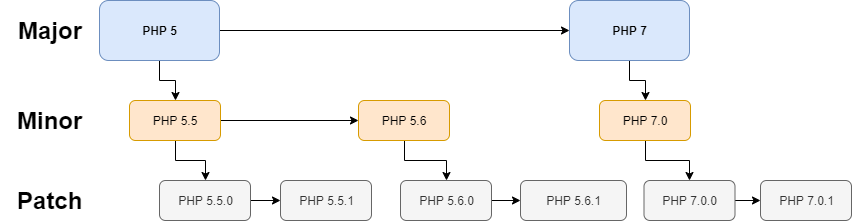
\includegraphics[width=1\linewidth]{gfx/semVer}} \quad
    \caption[Grafische Darstellung der Versionierung von PHP]{Grafische Darstellung der Versionierung von \acs{PHP}}\label{fig:semVer}
\end{figure}
